% Transition Diagrams for Exercise 3.4.1
% Author		: Finn Rayment
% Date created	: 17-03-2019
%

\documentclass{article}

\usepackage{tikz}
\usetikzlibrary{automata, positioning, arrows}

\begin{document}

\begin{figure}[ht]
\centering
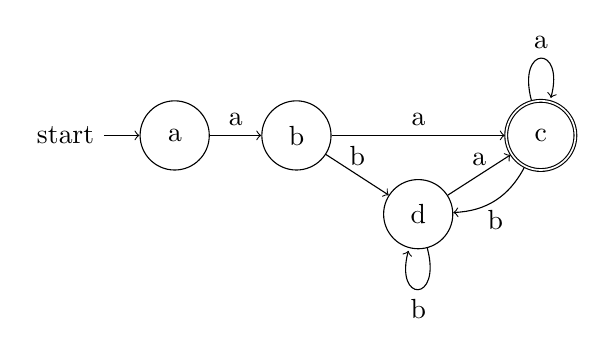
\begin{tikzpicture}%[bend angle=75]
	\node[state, initial] (q1) {a};
	\node[state, right of=q1, right=0.1cm] (q2) {b};
	\node[state, below of=q2, right of=q2, right=0.1cm] (q3) {d};
	\node[state, above of=q3, right of=q3, right=0.1cm, accepting] (q4) {c};

	\draw [->]
		(q1) edge[above] node{a} (q2)
		(q2) edge[above] node{b} (q3)
		(q2) edge[above] node{a} (q4)
		(q3) edge[above] node{a} (q4)

		(q3) edge[loop below] node{b} (q3)
		(q4) edge[loop above] node{a} (q4)

		(q4) edge[bend left, below] node{b} (q3)
		;
\end{tikzpicture}
\caption{a(a$\vert$b)*a}
\label{fig:a}
\end{figure}

\begin{figure}[ht]
\centering
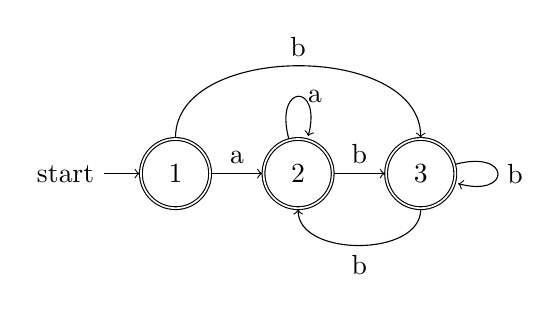
\begin{tikzpicture}[bend angle=90]
	\node[state, initial, accepting] (q1) {1};
	\node[state, right of=q1, right=0.1cm, accepting] (q2) {2};
	\node[state, right of=q2, right=0.1cm, accepting] (q3) {3};

	\draw [->]
		(q1) edge[above] node{a} (q2)
		(q2) edge[above] node{b} (q3)

		(q2) edge[loop above, right] node{a} (q2)
		(q3) edge[loop right] node{b} (q3)

		(q1) edge[bend left, above] node{b} (q3)
		(q3) edge[bend left, below] node{b} (q2)
		;
\end{tikzpicture}
\caption{(($\epsilon\vert$a)b*)*}
\label{fig:b}
\end{figure}

\begin{figure}[ht]
\centering
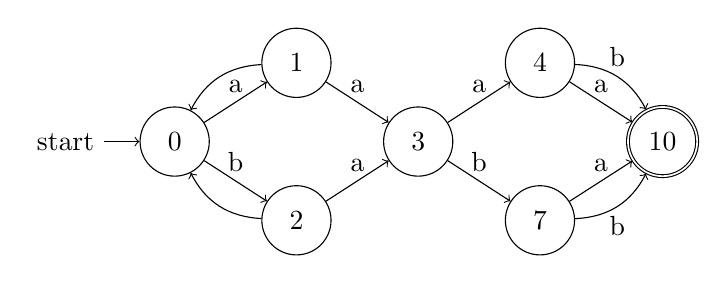
\begin{tikzpicture}
	\node[state, initial] (q1) {0};
		\node[state, above of=q1, right of=q1, right=0.1cm] (q2) {1};
		\node[state, below of=q1, right of=q1, right=0.1cm] (q3) {2};
	\node[state, below of=q2, right of=q2, right=0.1cm] (q4) {3};
		\node[state, above of=q4, right of=q4, right=0.1cm] (q5) {4};
		\node[state, below of=q4, right of=q4, right=0.1cm] (q6) {7};
	\node[state, below of=q5, right of=q5, right=0.1cm, accepting] (q7) {10};

	\draw [->]
		(q1) edge[above] node{a} (q2)
		(q1) edge[above] node{b} (q3)
		(q2) edge[above] node{a} (q4)
		(q3) edge[above] node{a} (q4)
		(q4) edge[above] node{a} (q5)
		(q4) edge[above] node{b} (q6)
		(q5) edge[above] node{a} (q7)
		(q5) edge[bend left, above] node{b} (q7)
		(q6) edge[above] node{a} (q7)
		(q6) edge[bend right, below] node{b} (q7)

		(q2) edge[bend right] node{} (q1)
		(q3) edge[bend left] node{} (q1)
		;
\end{tikzpicture}
\caption{(a$\vert$b)*a(a$\vert$b)(a$\vert$b)}
\label{fig:c}
\end{figure}

\begin{figure}[ht]
\centering
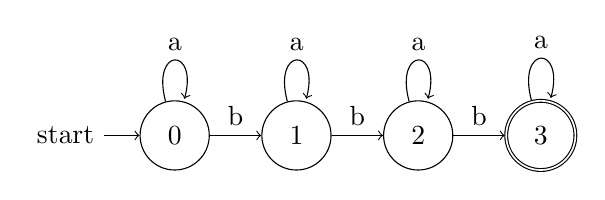
\begin{tikzpicture}
	\node[state, initial] (q1) {0};
	\node[state, right of=q1, right=0.1cm] (q2) {1};
	\node[state, right of=q2, right=0.1cm] (q3) {2};
	\node[state, right of=q3, right=0.1cm, accepting] (q4) {3};

	\draw [->]
		(q1) edge[above] node{b} (q2)
		(q2) edge[above] node{b} (q3)
		(q3) edge[above] node{b} (q4)

		(q1) edge[loop above] node{a} (q1)
		(q2) edge[loop above] node{a} (q2)
		(q3) edge[loop above] node{a} (q3)
		(q4) edge[loop above] node{a} (q4)
		;
\end{tikzpicture}
\caption{a*ba*ba*ba*}
\label{fig:d}
\end{figure}

\begin{figure}[ht]
\centering
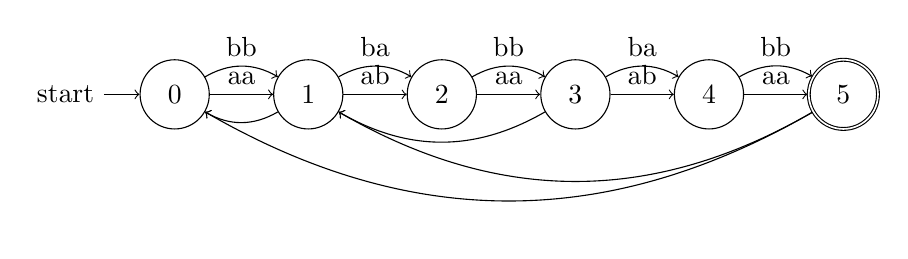
\begin{tikzpicture}bend angle=90]
	\node[state, initial] (q1) {0};
	\node[state, right of=q1, right=0.25cm] (q2) {1};
	\node[state, right of=q2, right=0.25cm] (q3) {2};
	\node[state, right of=q3, right=0.25cm] (q4) {3};
	\node[state, right of=q4, right=0.25cm] (q5) {4};
	\node[state, right of=q5, right=0.25cm, accepting] (q6) {5};

	\draw [->]
		(q1) edge[above] node{aa} (q2)
		(q2) edge[above] node{ab} (q3)
		(q3) edge[above] node{aa} (q4)
		(q4) edge[above] node{ab} (q5)
		(q5) edge[above] node{aa} (q6)

		(q1) edge[bend left, above] node{bb} (q2)
		(q2) edge[bend left, above] node{ba} (q3)
		(q3) edge[bend left, above] node{bb} (q4)
		(q4) edge[bend left, above] node{ba} (q5)
		(q5) edge[bend left, above] node{bb} (q6)

		(q2) edge[bend left] node{} (q1)
		(q4) edge[bend left] node{} (q2)
		(q6) edge[bend left] node{} (q2)
		(q6) edge[bend left] node{} (q1)
		;
\end{tikzpicture}
\caption{(aa$\vert$bb)*((ab$\vert$ba)(aa$\vert$bb)*(ab$\vert$ba)(aa$\vert$bb)*)*}
\label{fig:e}
\end{figure}

\end{document}
